\section{Object definitions and Event selection}

Events with at least one primary vertex passing an OR combination
of the HLTs shown on table \ref{tab:Datasets} containing at least three
electrons are selected provided that its missing energy $E_T^{Miss}$ is
greater than $40GeV$.

In addition, the following flags are required for the event (2016):

* Flag\_goodVertices
* Flag\_globalSuperTightHalo2016Filter
* Flag\_HBHENoiseFilter
* Flag\_HBHENoiseIsoFilter
* Flag\_EcalDeadCellTriggerPrimitiveFilter
* Flag\_BadPFMuonFilter

One additional flag is required for 2017, 2018:

* Flag\_ecalBadCalibFilterV2

Events are then splitted in four modes depending on the flavour and
number of leptons:

\begin{description}
\item[$\bullet$3e] $Z\rightarrow e^{+}e^{-} W\rightarrow e+\nu$
\item[$\bullet$2e+1mu] $Z\rightarrow e^{+}e^{-} W\rightarrow \mu+\nu$
\item[$\bullet$2mu+1e] $Z\rightarrow \mu^{+}\mu^{-} W\rightarrow e+\nu$
\item[$\bullet$3mu] $Z\rightarrow \mu^{+}\mu^{-} W\rightarrow \mu+\nu$
\end{description}


\subsection{High Level Trigger Selection}


\begin{table}[h]
\centering
\caption{List of HLT requirements and its associated dataset.}
\begin{tabular}{|l|l|l|}
\hline
Year & Dataset & HLT                \\ \hline
2016 & SingleMuon     & HLT\_TkMu50 \\
     &                & HLT\_Mu50   \\
     & SingleElectron & HLT\_Ele27\_WPTight\_Gsf  \\
     & SinglePhoton   & HLT\_Photon175            \\ \hline
2017 & SingleMuon     & HLT\_Mu50       \\
     &                & HLT\_OldMu100   \\
     &                & HLT\_TkMu100    \\
     & SingleElectron & HLT\_Ele35\_WPTight\_Gsf  \\
     & SinglePhoton   & HLT\_Photon200            \\ \hline
2018 & SingleMuon & HLT\_Mu50     \\
     &            & HLT\_OldMu100 \\
     &            & HLT\_TkMu100  \\ \hline
     & EGamma     & HLT\_Ele32\_WPTight\_Gsf \\
     &            & HLT\_Photon200           \\ \hline
\end{tabular}
\label{tab:Datasets}
\end{table}


\subsection{Lepton Selection}

\subsection{Electrons}

Electrons are reconstructed from the different hits in the different
layers of the tracker and energy deposits in the scintillating crystalls
across the $\eta-\phi$ plane in the Electromagnetic Calorimeter.

The electron's sign charge can be identified by its signature in the tracker
due to the presence of the strong magnetic field in the CMS detector.

Electrons are required to be within the ECAL fiducial region i.e
$\abs{eta}<2.5$ excluding the transition region betwen the barrel and
the endcaps $1.4442<\abs{eta}<1.5660$.

\subsection{Muons}

When compared to electrons, muons are reconstructed more efficiently due to additional
additional hits collected in the muon chambers.
In the same way that the electron tracks, the muon tracks are bent due to the
the presence of the strong magnetic field. However, as
muons posess a longer lifetime they travel a longer distance in the detector and
its tracks are able to reflect the change of sign in the magnetic field after
its passage through the superconducting solenoid.

The muon objects in this analysis can be divided into two categories:
Tracker and Global muons.

Muons are required to be within the pseudorapidity range $\abs{eta}<2.4$ and
to have a minimum transverse momentum of $P_t=20$. Additionally the leading muon of
the event is required to have $P_t>52$ in line with the trigger plateau.


\subsection{Z Candidate}

Two same flavored, opposite signed leptons are required to reconstruct a Z
candidate. If more than one pair is found, the one with reconstructed mass
closer to the nominal mass $M_z= 91.1876 GeV$ is chosen. The pair's mass
is required to fall in the Z mass window $ 70. GeV < M_Z < 111. $.

If the Z candidate is formed from a muon pair with a leading (subleading) muon with
a transverse momentum of at least $P_t=70 GeV$ ($P_t=10GeV$). One of the
muons is required to pass two additional requirements: being a global high-Pt muon and a
particle-flow candidate. In the case of electrons, the requirement is to have
a transverse momentum of at least $P_t=27GeV$ (2016) matching the trigger
plateau, $P_t=35GeV$ (2017), $P_t=32GeV$ (2018).

The event is rejected if the the distance in the $\eta-\phi$ plane for the two
leptons product of the decay of the Z is less than $1.5$.




\subsection{W Candidate}

The neutrino coming from The $W \rightarrow l\nu$ candidate escapes undetected,
and therefore the following assumptions are made in order to perform a kinematic
reconstruction of the $W$ candidate: there is no additional sources of missing
energy, and consequently $E_{Pt}^{miss}$ is considered the transverse momentum
corresponding to the undetected neutrino. The longitudinal momentum $P_z$ can be
recovered by imposing the $M_W = 80.379 GeV $ nominal mass and $M_\nu = 0.$

$W$ boson is reconstructed from the remaining lepton
and the missing energy $E_T^{miss}$. The ramining lepton is required to be either
a tight electron or a global High-Pt muon with a transverse momentum of at least
$Pt=50GeV$


\subsection{WZ Candidate}

* Mass of the three leptons system should be greater than $120GeV$
* The sum of the transverse momentum of the leptons should be greater than $110GeV$









\begin{figure}[tph]
  \centering
        \subfigure[2016]{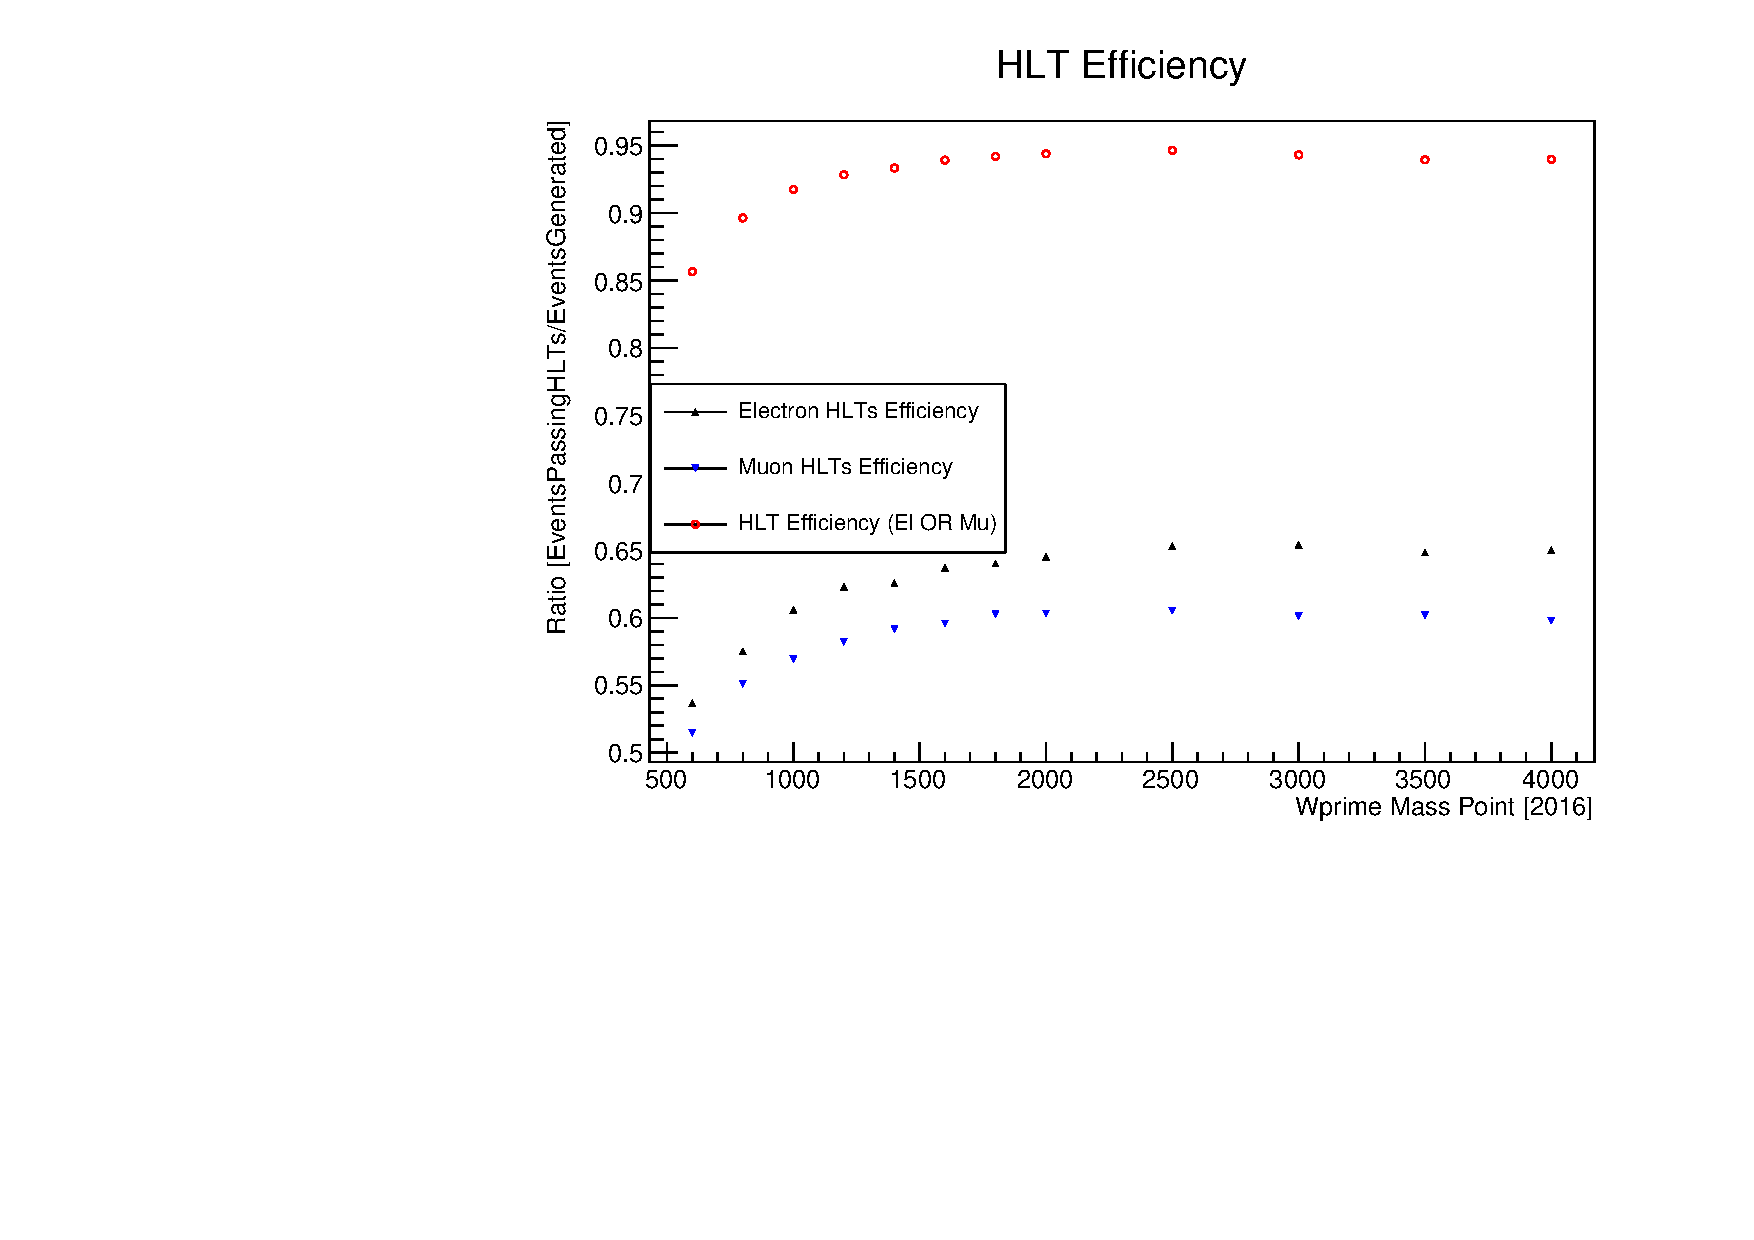
\includegraphics[width=.28\textwidth]{fig/2016_SignalTriggerEfficiency.pdf}}
        \subfigure[2017]{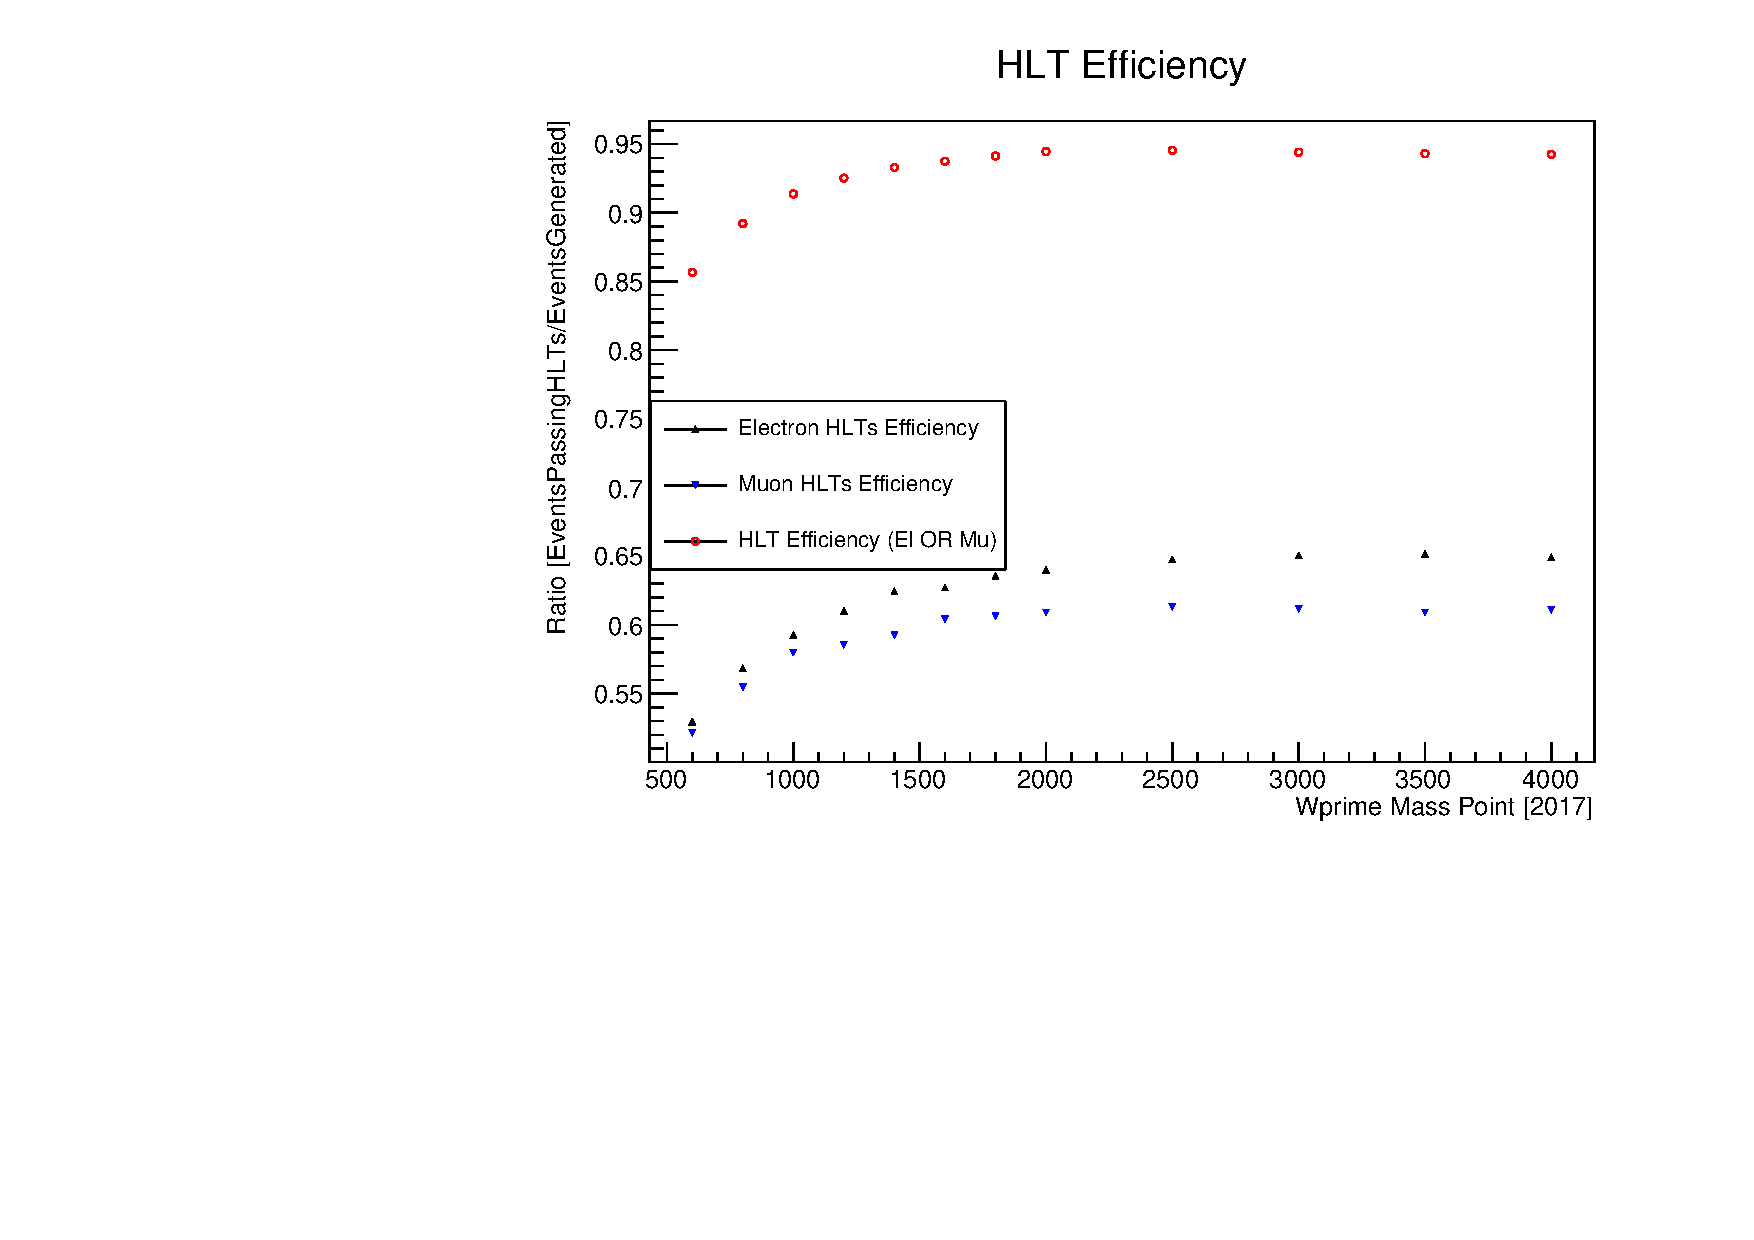
\includegraphics[width=.28\textwidth]{fig/2017_SignalTriggerEfficiency.pdf}}
        \subfigure[2018]{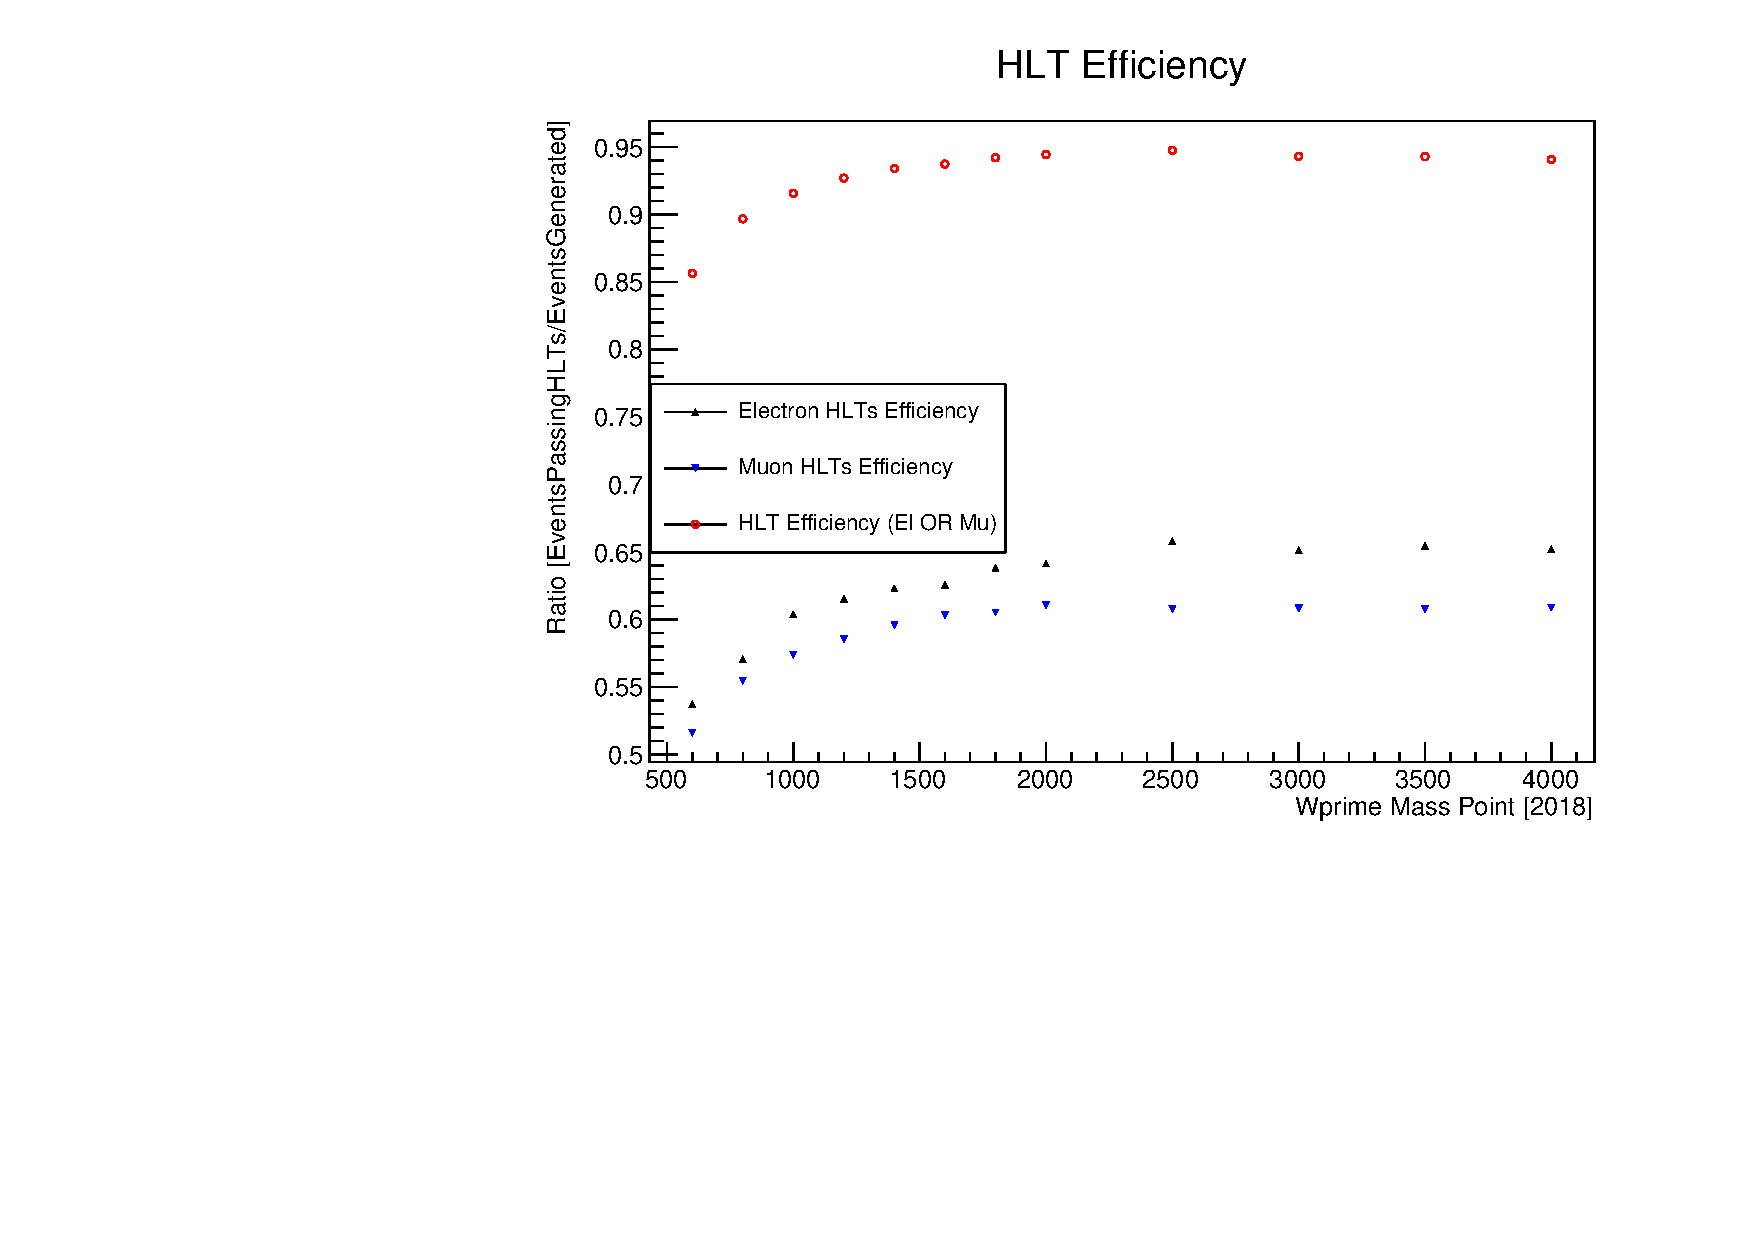
\includegraphics[width=.28\textwidth]{fig/2018_SignalTriggerEfficiency.pdf}}
  \caption{Signal efficiency for individual and combined High Level Triggers for Run II}
  \label{fig:hltSignalEfficiency}
\end{figure}

